\chapter{INTRODUCTION}

\section{Systems Biology}

With the increasing availability of the computational tools and the development of high throughput techniques in the omics field, systems biology has shown a strong emergence in the last few years as a key multi-disciplinary field for integrating the multi-layer complexity of biological systems, particularly in the areas of transcriptomics, proteomics, metabolomics and fluxomics \cite{kitano2002systems}. This amount of available data allows researchers to investigate molecular cell processes in a large scales, applying theoretical, experimental and computational methods.

Biological systems based on complex interactions between various molecular components. The relations between these components are often obey nonlinear kinetics, for example, most of the reactions are regulated by one or more feedback or feed-forward loops with incomprehensible behaviours. When considered, cell structure and compartmentalization are also often introduce complexities to the unexpected behavior of the entire biological system \cite{bellouquid2006mathematical}. Mathematical modeling with these factors taken into consideration is used as a general approach to encompass existing knowledge in biological systems, and to gather information by analyzing these models to acquire a better understanding \cite{kremling2013systems}.


A mathematical model of a cell can be approached by two different approaches in either a bottom-up or top-down directionality (Figure \ref{fig:systemsbiology}) \cite{bruggeman2007nature, shahzad2012application}. Top-down approach is an experimental oriented approach, it starts from the whole picture and aims to characterize biological mechanisms closer to the smaller parts and their interactions in the network. In the bottom-up approach, collected data from biological knowledge is used as a starting point, a subsystem is generated to deduce the functional properties of smaller points in the network. Combination of the pathway level models (bottom-up) into a model for the entire system level (top-down) is the ultimate goal in the systems biology therefore these approaches are complementary.

\begin{figure}[ht]
\begin{center}
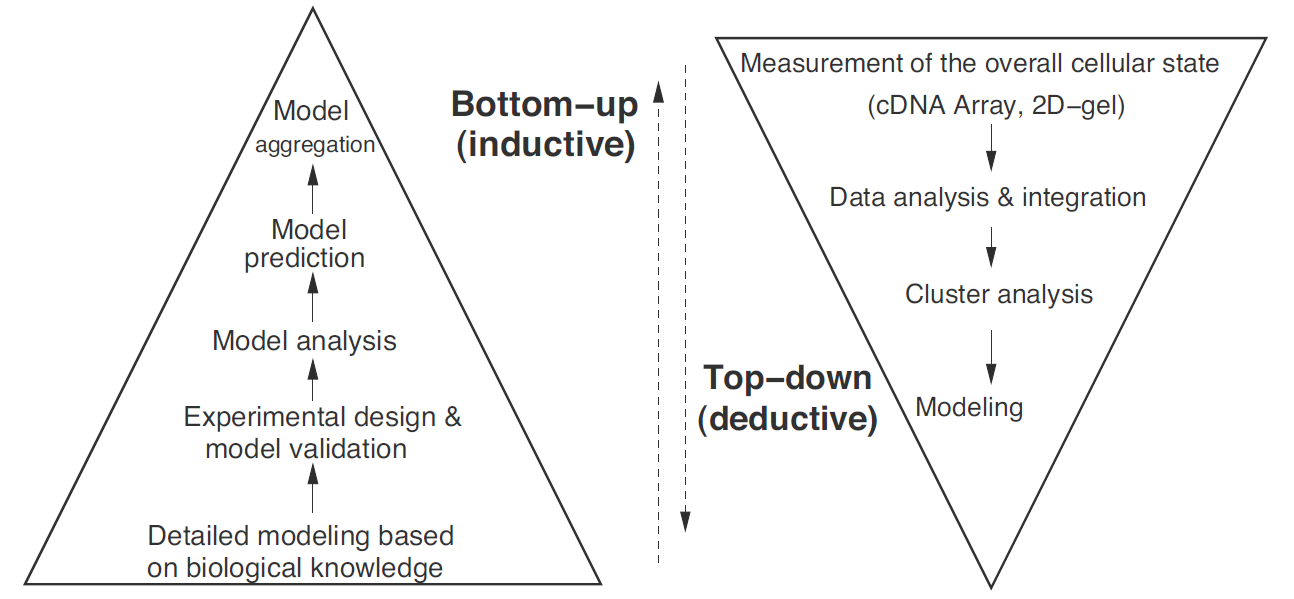
\includegraphics[width=0.8\columnwidth]{systemsbiology.png}
\end{center}
\caption{Systems biology approaches. Left: Bottom-up approach. Right: Top-down approach. Figure is taken from \cite{kremling2013systems}.}
\vskip\baselineskip % Leave a vertical skip below the figure
\label{fig:systemsbiology}
\end{figure}

\subsection{Metabolic Networks}
In the context of systems biology, metabolic network reconstructions have become a common denominator over the past 10 years \cite{thiele2010protocol}. Organism-specific metabolic network analyses allow scientists to design experiments and even obtain beforehand predictions. These networks are the main sources of the mathematical models which can simulate metabolic fluxes reflecting the experimantal reality \cite{orth2010flux}.

A generally applicable protocol is defined by the Palsson group \cite{thiele2010protocol, feist2009reconstruction} for the reconstruction of biochemical networks described in the Figure \ref{fig:modelreconstruction} \cite{chen2012metabolic}). Briefly, genomic data for the biochemical reactions of an organism are identified from the databases, such as NCBI, DDBJ and EMBL-EBI. Since the genomic data is the least representative of the biological phenotypes; available transcriptomic, proteomic, metabolomic and/or subcellular localization data are also used to further curate the model. Once the final metabolic network is reconstructed, it is translated into a mathematical model and validated by the experimental data.

\begin{figure}[ht]
\begin{center}
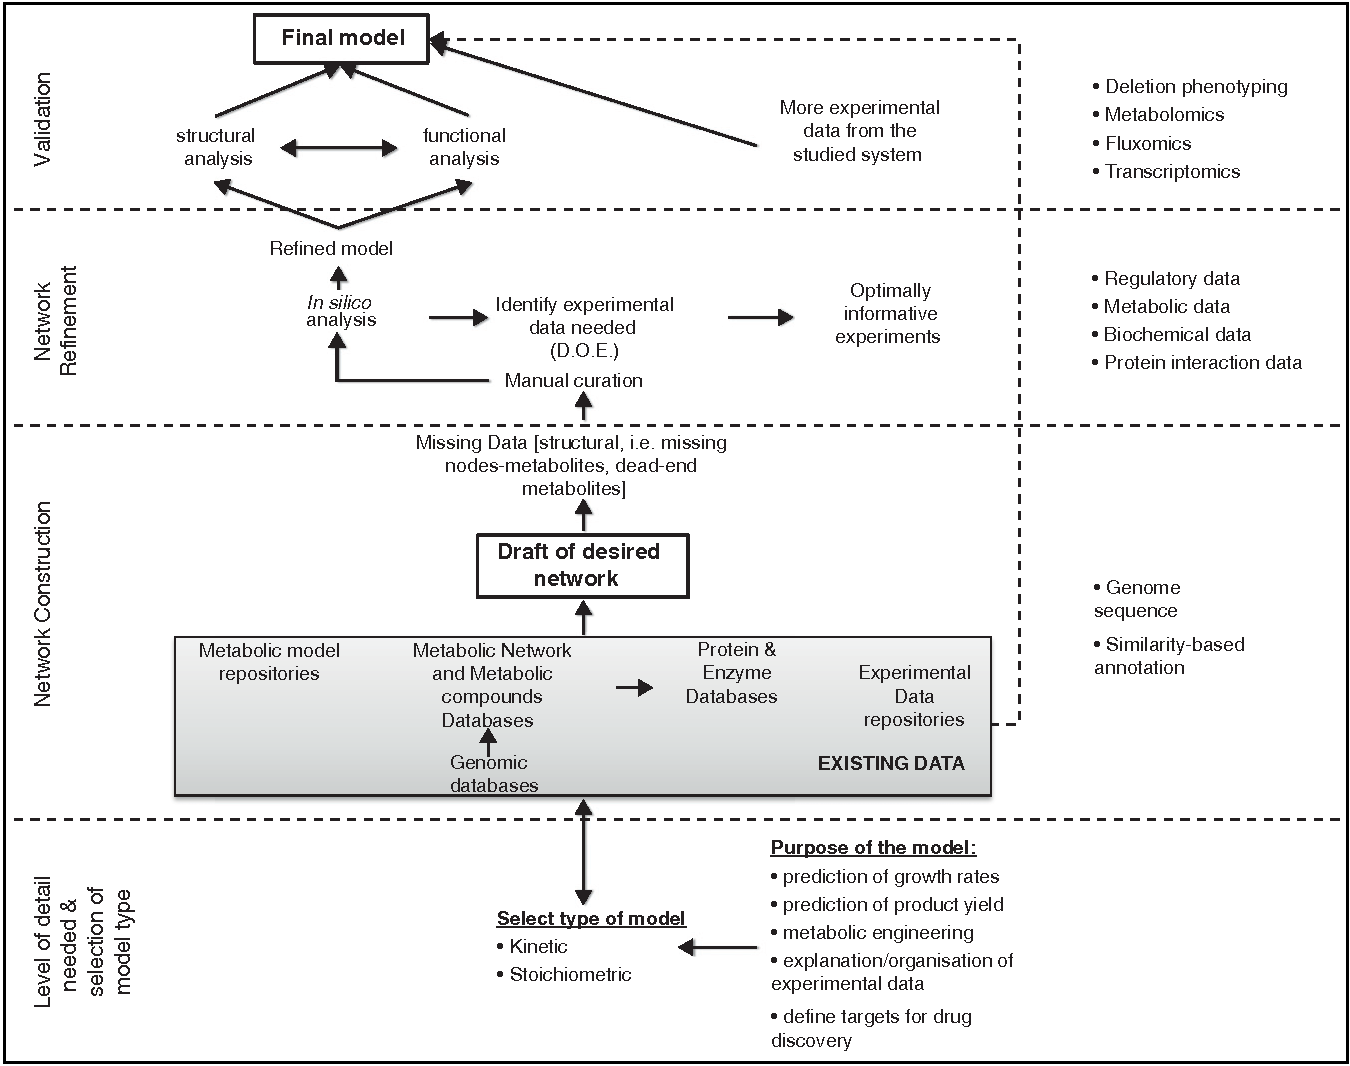
\includegraphics[width=1\columnwidth]{modelreconstruction.png}
\end{center}
\caption{Overview of metabolic network reconstruction protocol. Figure is taken from \cite{chen2012metabolic}.}
\vskip\baselineskip % Leave a vertical skip below the figure
\label{fig:modelreconstruction}
\end{figure}

Once a metabolic network is reconstructed, a rational link between a genome sequence, the proteins encoded in the genome, and the reactions catalyzed by the proteins allowing to investigate the relationships between genotype and phenotype is achieved \cite{durot2008genome}.

Approaches for analyzing metabolic networks are mainly categorized as dynamic or structural approaches. Even though the former is promising more realistic approach, its implementation in the literature is obstructed due to the unavailability of kinetic parameters for the majority of enzymes within a metabolic network \cite{machado2014systematic, ramkrishna2012dynamic} Because of the lack of kinetic parameters, structural metabolic modeling has been widely used for analyzing cellular metabolism at a steady-state assumption.

\subsection{Mathematical Representation of Metabolic Networks}
\hl{There will be a review on} "Mathematical Framework Behind the Reconstruction and Analysis of Genome Scale Metabolic Models" \cite{pinzon2018mathematical})

In a stoichiometric matrix, each column is a reaction in the network and each of the rows is associated with a component or metabolite expressed by its stoichiometric coefficient, being negative if it is a reactant from the perspective of the reaction...

\subsection{Flux Balance Analysis}
\hl{There will be a review on} "What is flux balance analysis?" \cite{orth2010flux}

\section{\emph{Saccharomyces cerevisiae}}
\subsection{Industrial importance of \emph{S. cerevisiae}}
\subsection{Metabolic Models of \emph{S. cerevisiae}}
\subsection{Applications of \emph{S. cerevisiae} GSMMs}

\section{Significance of Thesis}
